\chapter{Reconfigurable computing e \acs{FASTER}}
\label{chap:recComputingFASTER}
\vspace{1cm}
Questo capitolo spiega pi\`u dettagliatamente la fase di
riconfigurazione, introdotta nel capitolo \ref{chap:intro}, e presenta il
framework sviluppato presso il Politecnico di Milano per il progetto
europeo \acs{FASTER}, nel quale trova collocamento questo lavoro di tesi.

La sezione \ref{sec:recComputingDettagli} descrive i vari tipi di
riconfigurazione e il processo di riconfigurazione dei chip \ac{FPGA}.

La sezione \ref{sec:progettoFASTER} presenta un esempio di framework per il
design di \ac{MPSoC} riconfigurabili, il progetto europeo \acs{FASTER},
all'interno del quale si colloca il lavoro su mapping e scheduling oggetto di questa
tesi. Viene presentata la metodologia proposta per la toolchain e l'algoritmo
che effettua l'analisi esplorativa delle soluzioni, che interagisce con lo
scheduler.

\newpage

\section{Tipi e processo di riconfigurazione}
\label{sec:recComputingDettagli}
In questa sezione vengono descritti i tipi di riconfigurazione e viene introdotta
la nozione di \emph{dimensione} della riconfigurazione. L'ultima parte della sezione
spiega brevemente come avviene il processo di riconfigurazione di un chip \ac{FPGA}.
\subsubsection{Tipi di riconfigurazione}
Inizialmente, il reconfigurable computing veniva utilizzato per realizzare prototipi
economici di soluzioni hardware, mentre oggigiorno non \`e raro trovare in commercio
controllori basati su \ac{FPGA}. I continui progressi tecnologici hanno portato infatti
a un'evoluzione della fase di riconfigurazione. Le possibilit\`a di usufruire della
riconfigurazione sono passate dal poter riconfigurare un dispositivo solamente una volta,
prima di eseguire l'applicazione, al poter riconfigurare in maniera trasparente alcune porzioni
della logica, consentendo ad altri moduli di proseguire la loro esecuzione in parallelo.
I vari tipi di riconfigurazione sono i seguenti:
\begin{itemize}
 \item \emph{riconfigurazione totale}: il dispositivo viene riconfigurato e durante
   il processo tutti i dati presenti vengono cancellati;
 \item \emph{riconfigurazione parziale}, che a sua volta si divide in:
     \begin{enumerate}
        \item \emph{statica}: il dispositivo può essere riconfigurato
interrompendo temporaneamente l'esecuzione dell'applicazione;
        \item \emph{dinamica}, in inglese \acf{DPR}: parte della logica
può essere riconfigurata tramite un bitstream parziale, senza interrompere i task in
esecuzione su altre regioni del dispositivo.
    \end{enumerate}
\end{itemize}
L'utilizzo della riconfigurazione parziale dinamica rappresenta il motivo per cui le
architetture riconfigurabili possono adattarsi in maniera dinamica al carico di lavoro richiesto,
oppure a sopperire a eventuali guasti o ancora a poter eseguire applicazioni pi\`u complesse
senza che il requisito in termini di area del \emph{die} aumenti.

\begin{figure}[t]
 \begin{minipage}[b]{0.4\textwidth}
  \begin{center}
   $\vcenter{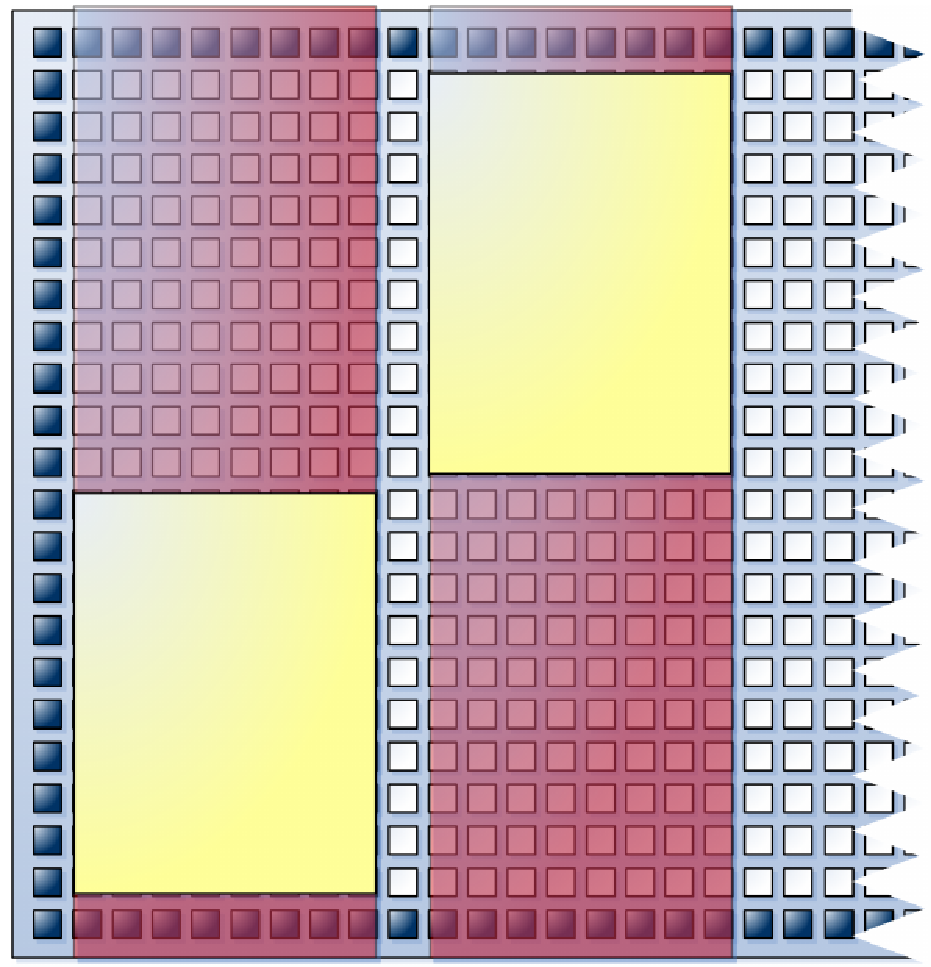
\includegraphics[width=0.7\linewidth]
{capitoli/figure/cap2/Riconfigurazione1D.pdf}}$
  \end{center}
 \end{minipage}
 \hfill
 \begin{minipage}[b]{0.4\textwidth}
 \begin{center}
    $\vcenter{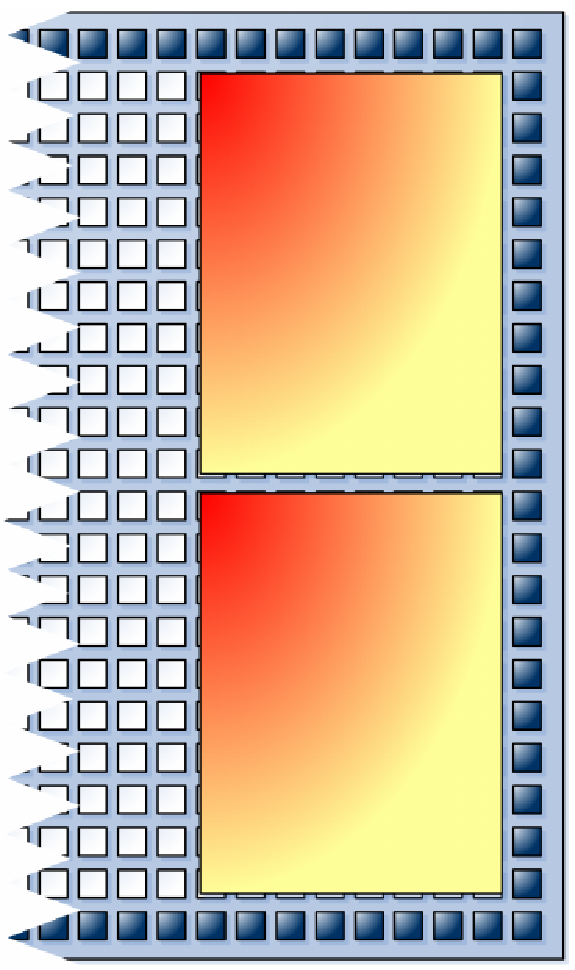
\includegraphics[width=0.45\linewidth]
{capitoli/figure/cap2/Riconfigurazione2D.pdf}}$
 \end{center}
 \end{minipage}
 \caption[Riconfigurazione 1D e 2D]{Riconfigurazione 1D e 2D \cite{Redaelli2DILP}.}
 \label{fig:riconfigurazione1D2D}
\end{figure}


\subsubsection{Riconfigurazione a due dimensioni}
Le schede \ac{FPGA} moderne supportano la riconfigurazione parziale dinamica a due dimensioni,
che permette di aumentare il grado di libertà del designer.

La differenza tra la riconfigurazione a singola dimensione (per colonne) e la
riconfigurazione a due dimensioni è mostrata in figura~\ref{fig:riconfigurazione1D2D}.
Nella riconfigurazione a una dimensione, un modulo che occupa soltanto parte di una
colonna richiede la riconfigurazione di tutta la colonna, il che proibisce il piazzamento
di altri moduli in colonne sovrapposte al primo. La riconfigurazione a due dimensioni
permette, invece, di piazzare i due moduli in un'area della scheda molto più compatta e di
incrementare potenzialmente il numero di moduli che possono essere accelerati se eseguiti
su logica riconfigurabile. Inoltre, poich\'e a parit\`a di requisiti del modulo l'area da
riconfigurare nel caso a due dimensioni \`e minore, i tempi necessari per eseguire
le riconfigurazioni si riducono.

L'aumento di versatilità derivante dall'uso della riconfigurazione parziale dinamica
a due dimensioni comporta un notevole sforzo da parte del designer del sistema,
che deve capire quando usare la riconfigurazione permetta un guadagno di prestazioni
e quali moduli riconfigurare, oltre a come piazzare fisicamente questi moduli per sfruttare al
meglio l'area a disposizione.

\subsubsection{Bitstream e processo di riconfigurazione}
Il bitstream è un file binario che contiene i dati da copiare nelle celle di memoria RAM
statica che contengono la configurazione. In un'architettura provvista di
riconfigurazione parziale dinamica, il bitstream può essere di due tipi:
\begin{itemize}
 \item completo, utilizzato per l'inizializzazione della configurazione del dispositivo;
 \item parziale, che configura soltanto alcune porzioni dell'area riconfigurabile.
\end{itemize}

La configurazione avviene per mezzo di interfacce, che variano a seconda dell'\ac{FPGA}
che si utilizza: un'interfaccia può essere basata su microcontrollori, sul caricamento
della configurazione da schede compact flash, su un \ac{ICAP}, etc.

A prescindere dal tipo di interfaccia utilizzato, il dispositivo possiede una
\emph{logica di configurazione}, che interpreta il bitstream per poter configurare
il dispositivo. Lo stato di tale logica è salvato all'interno di un insieme di \emph{registri di configurazione}.
I dati sulla configurazione vengono scritti dal bitstream a questi registri e successivamente
vengono copiati dalla logica di configurazione nelle memorie statiche.


\section[Il progetto \acs{FASTER}]{Il progetto \acs{FASTER}}
\label{sec:progettoFASTER}
In questa sezione vengono presentati il fondamento logico e le motivazioni alla 
base del progetto \acs{FASTER}. La sezione~\ref{subsec:fasterIntro} fornisce 
un'introduzione al progetto e spiega gli obiettivi e le motivazioni alla 
base che hanno portato alla creazione del progetto; infine, la
sezione~\ref{sec:fasterMetodologia} illustra la metodologia tramite la quale si possono 
raggiungere gli obiettivi prefissati.


%%% acro definitions
\acrodef{NIDS}{Network Intrusion Detection System}
\acrodef{RTM}{Reverse Time Migration}
\acrodef{TCO}{Total Cost of Ownership}
\acrodef{ICS}{Institute of Computer Science}
\acrodef{FORTH}{Foundation for Research and Technology - Hellas}
%%%%%%%%%%%%%%%%%%%%%%%%%%%%%%%%%%%%%%

% mark FASTER acronym as used
\acused{FASTER}

\subsection{Introduzione}
\label{subsec:fasterIntro}
\acs{FASTER} è l'acronimo di \emph{\acl{FASTER}}, un progetto\footnote{Sito del 
progetto: \url{http://www.fp7-faster.eu/}.} organizzato dalla comunità europea 
che coinvolge diverse aziende e atenei,\footnote{I collaboratori del progetto 
sono: l'\ac{ICS} di \ac{FORTH} in Grecia, Chalmers University of Technology in 
Svezia, l'università di Ghent in Belgio, l'Imperial College di Londra, il 
Politecnico di Milano e le aziende Maxeler, ST Microelectronics e Synelixis.} 
tra cui il Politecnico di Milano. Il progetto è stato avviato l'1/09/2011,
ha una durata di 36 mesi ed è supportato tramite fondi stanziati dalla 
comunità europea.

\subsubsection{Motivazioni e obiettivi del progetto}
L'ambito di applicazione del progetto \ac{FASTER} sono le architetture 
riconfigurabili; in particolare \ac{FASTER} è pensato, come il nome 
suggerisce, per facilitare la definizione e l'uso di sistemi implementati in 
hardware riconfigurabile \cite{FasterPaper}.

Sfruttando le potenzialità delle promettenti architetture hardware basate sulla 
logica riconfigurabile, introdotte nel capitolo~\ref{chap:intro}, si possono 
infatti estendere le funzionalità (e quindi la durata utile della vita) di 
un'applicazione senza dover riprogettare interamente l'hardware necessario per 
eseguirla.

Nonostante il vantaggio di utilizzare architetture riconfigurabili rispetto 
all'eseguire le applicazioni puramente in software, il design e 
l'implementazione di un sistema basato su logica riconfigurabile hanno delle 
limitazioni rispetto alla più facile estensione delle funzionalità di 
un'applicazione software, per le seguenti ragioni:
\begin{itemize}
 \item il supporto di tool esterni per il design del sistema è ancora limitato;
 \item le riconfigurazioni hanno un considerevole impatto in termini di overhead sul 
tempo di esecuzione dell'applicazione, pertanto devono essere utilizzate con 
attenzione;
 \item la gestione delle risorse disponibili sulla scheda (anche a run-time) è 
interamente affidata all'utente.
\end{itemize}
Oltre a queste limitazioni, il designer ha altri compiti da assolvere per 
implementare correttamente un sistema su hardware riconfigurabile, tra cui 
l'identificazione di quali parti del codice devono essere eseguite in hardware 
per avere un effettivo guadagno in termini di velocità di esecuzione, quali 
moduli hardware possono beneficiare di una riconfigurazione, stabilire uno 
schedule e verificare la bontà della soluzione così ottenuta.

Il progetto \ac{FASTER} concentra dunque i propri obiettivi nell'introduzione 
di una nuova metodologia che permetta ai designer di implementare facilmente un 
sistema su una piattaforma target dotata di processori general-purpose e 
acceleratori hardware basati su logica riconfigurabile. Questa metodologia 
consentirà, partendo da un input costituito da una descrizione ad alto livello 
sia dell'applicazione che dell'architettura, di sfruttare al massimo le 
possibilità offerte dalla riconfigurazione parziale dinamica.

\paragraph{Lavori precedenti}
Tra i lavori di ricerca e progetti europei più vicini a \ac{FASTER} si 
annoverano \emph{hArtes} \cite{HArtes}, \emph{Morpheus}, \emph{ACOTES} 
\cite{AcotesUrl, ACOTES}, \emph{Andres} e \emph{Reflect} \cite{Reflect}.
% FIXME citazioni mancanti perchè i siti sono offline
Questi lavori hanno obiettivi simili a quelli di \ac{FASTER}, tuttavia si 
concentrano più sugli aspetti architetturali della riconfigurazione; in questi 
lavori non si accenna esplicitamente al design della riconfigurazione parziale 
dinamica, nè si considera quale granularità sia meglio utilizzare per la 
riconfigurazione. 
%\emph{region-based}\footnote{Nella riconfigurazione di tipo 
%region-based, sono riconfigurati interi moduli che occupano arbitrarie porzioni 
%della scheda.} oppure \emph{micro-riconfigurazione}\footnote{Nella 
%micro-riconfigurazione vengono identificati dei parametri del modulo che 
%sono soggetti a cambiamenti; tali parametri non vengono inclusi nel bitstream, 
%lasciando così dei ``buchi''. Quando i valori per tali parametri devono essere 
%fissati, è sufficiente lanciare una riconfigurazione con un bitstream di 
%dimensioni molto ridotte, che vada a modificare solamente i buchi lasciati in 
%precedenza.}.

%TODO aggiungere tabella presente nel paper su dprds

\paragraph{Contributi di \ac{FASTER}}
\ac{FASTER} si distingue rispetto ai lavori precedentemente sviluppati in 
quanto ha come obiettivo l'introduzione della riconfigurazione parziale 
dinamica come un concetto di design esplicito, fornendo anche i metodi per 
supportare la riconfigurazione a run-time nell'intera metodologia di design.
Il progetto \ac{FASTER} quindi, possiede le seguenti caratteristiche:
\begin{enumerate}
 \item fornisce supporto per la riconfigurazione parziale 
dinamica, in maniera trasparente 
all'utente;
 \item fornisce un framework per il design di un sistema su logica 
riconfigurabile, gestendo l'analisi, la sintesi e la verifica delle soluzioni 
ottenute.
\end{enumerate}

Gli obiettivi che il progetto \ac{FASTER} si prefigge di raggiungere sono un 
significativo aumento della produttività nel design e nell'implementazione di 
sistemi riconfigurabili, aumento delle performance delle applicazioni 
sviluppate in hardware in presenza di vincoli sul consumo energetico e 
riduzione del costo totale di proprietà\footnote{In inglese \emph{\ac{TCO}}, 
rappresenta l'insieme di tutti i costi da sostenere per l'intero ciclo di 
vita di un sistema o un'apparecchiatura IT.} per sistemi come \ac{NIDS} e 
\ac{RTM} \cite{RTMArticle} implementati su hardware riconfigurabile, grazie alla minore 
manutenzione richiesta. Come scritto dagli autori nel factsheet di \ac{FASTER}
\cite{FasterFactsheet}

\selectlanguage{english}

\begin{quotation}
  \ac{FASTER} will facilitate the use of reconfigurable technology by providing a complete
  methodology that enables designers to easily implement and verify applications on
  platforms with general-purpose processors and acceleration modules implemented in the
  latest reconfigurable technology.
  We expect that the 
  project will lead to a 20\% productivity improvement due to seamless 
  implementation and verification of dynamically changing systems, a 50\% total 
  ownership cost reduction for NIDS and Reverse Time Migration systems, with a 2x 
  performance improvement under power constraints for Global Illumination and 
  Image Analysis.
\end{quotation}

\selectlanguage{italian}

Nella prossima sezione verr\`a illustrata la metodologia proposta per il framework. 


\subsection{Descrizione del framework}
\label{sec:fasterMetodologia}


\begin{figure}
 \begin{center}  
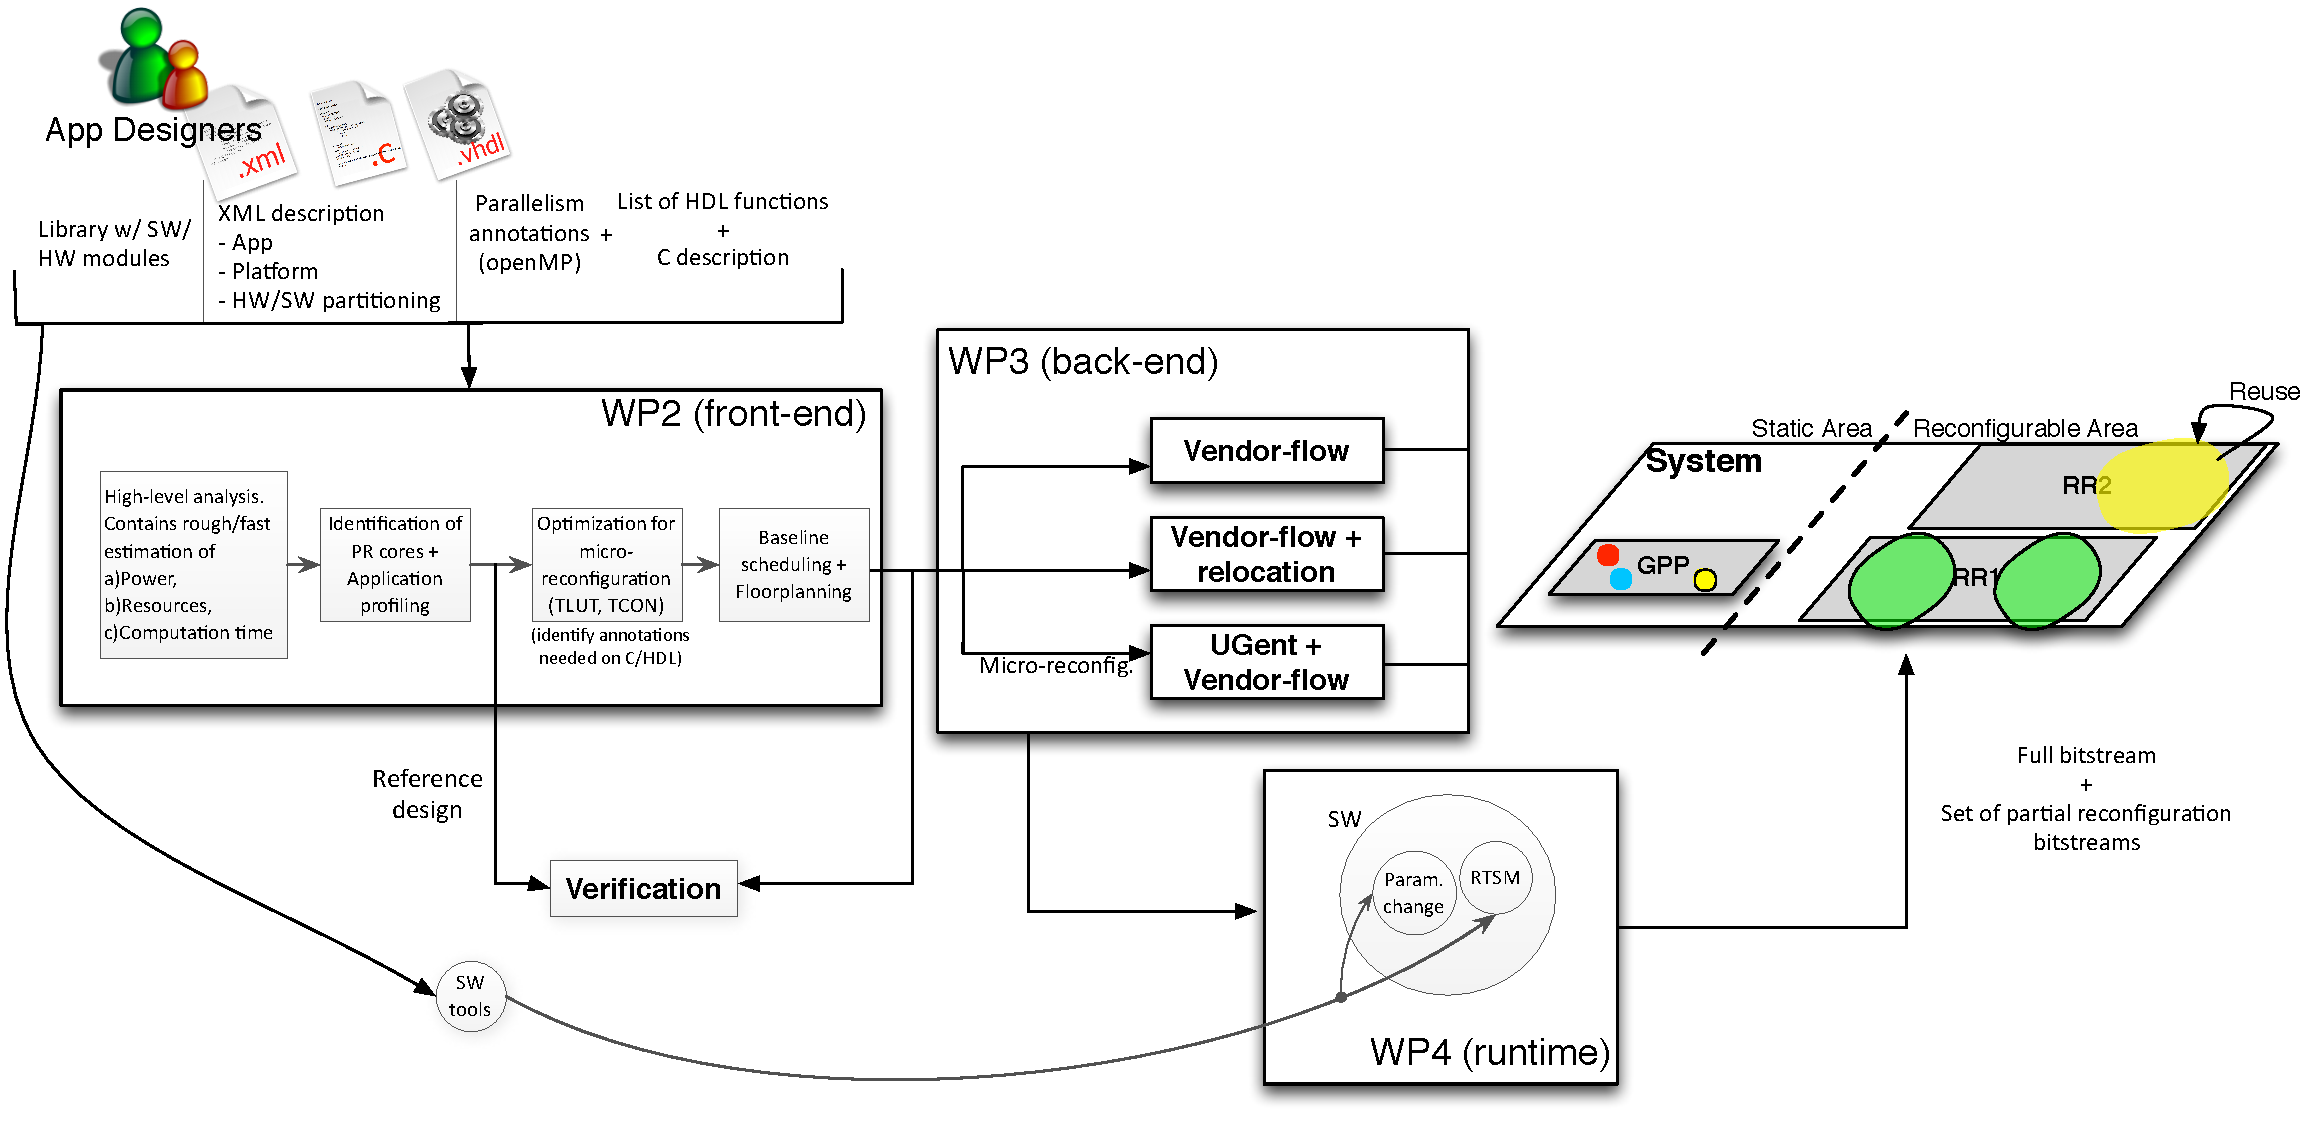
\includegraphics[width=\textwidth]
{capitoli/figure/cap2/FASTERWorkflow.pdf}
\caption[Workflow di \acs{FASTER}]{Workflow di \acs{FASTER} \cite{FasterApproach}.}
\label{fig:FASTERWorkflow}
 \end{center}
\end{figure}

La figura~\ref{fig:FASTERWorkflow} illustra la panoramica della metodologia 
adottata da \ac{FASTER} e il flusso di lavoro che, partendo dalla specifica 
dell'applicazione annotata e dalla descrizione dell'architettura target, riesce 
a derivare un bitfile utilizzabile per configurare l'architettura ed eseguire 
l'applicazione tramite un runtime manager.

L'approccio adottato da \ac{FASTER} prevede che i vari componenti del framework
si interfaccino tra loro mediante l'uso di file XML. L'input di un progetto
\ac{FASTER} è costituito dall'applicazione da sintetizzare, che può essere
scritta in un linguaggio ad alto livello (ad esempio il linguaggio C) e
provvista di annotazioni, ad esempio in formato OpenMP,\footnote{OpenMP è un
  formato standard per la specifica di applicazioni parallele, che permette di
  specificare quali funzioni di un'applicazione sono parallelizzabili e di
suddividere l'applicazione nei vari task.} che ne consentono la suddivisione
iniziale in task; altro dato in input \`e la descrizione delle funzionalità di
riconfigurazione a disposizione dell'architettura. Oltre all'applicazione
possono essere presenti degli attributi specificati dal designer che impongono
vincoli particolari all'applicazione, quali ad esempio scadenze nell'esecuzione
oppure una richiesta in termini di throughput.

\paragraph{High-level analysis}
La prima fase del flusso di lavoro prevede l'analisi ad alto livello 
dell'applicazione e dei suoi requisiti. In questa fase è fornito un modello di 
design riconfigurabile che mette in relazione i requisiti dell'applicazione con 
determinate metriche di valutazione delle performance.

Tramite questo processo si possono identificare dei componenti e determinare le 
performance delle relative implementazioni: esempi di parametri relativi a
un'implementazione sono le stime di risorse occupate, dell'overhead introdotto 
dalle riconfigurazioni o del consumo di energia in base all'area occupata su 
scheda.

\paragraph{Identificazione dei core}
Durante questa fase viene analizzata l'applicazione per estrarne i vari core, 
ovvero moduli composti da una serie di operazioni. I moduli sono estratti 
partendo dal \ac{CDFG} dell'applicazione; è possibile 
riutilizzare uno o più moduli, se la loro funzionalit\`a \`e equivalente,
senza fare uso di riconfigurazione e guadagnando 
quindi in termini di tempo di esecuzione.
I core possono essere di due tipi:
\begin{enumerate}
 \item \emph{statici}, moduli configurati staticamente e non soggetti a
   riconfigurazioni durante l'esecuzione (ad esempio core IP);
 \item \emph{riconfigurabili}, i quali a loro volta si dividono in:
  \begin{itemize}
   \item \emph{region-based}, in cui l'intero modulo viene riconfigurato;
   \item \emph{micro-riconfigurabili}, in cui solo piccole parti del modulo 
     sono riconfigurate e il resto viene riutilizzato \cite{FPGAReconfigurationGhent}.
  \end{itemize}
\end{enumerate}

Al termine dell'identificazione dei core, si svolge la fase di 
\emph{partitioning}, in cui si stabilisce quali parti dell'applicazione debbano 
essere eseguite in software su un processore general-purpose e quali in 
hardware su logica riconfigurabile.

\paragraph{Baseline scheduling}
A questo punto, partendo dalle informazioni calcolate nei passi precedenti, 
viene calcolato un baseline schedule dei task sulla piattaforma target. Lo 
schedule viene calcolato da uno scheduler euristico che deve essere consapevole
delle riconfigurazioni che vengono introdotte. Lo scheduler deve quindi 
avere le seguenti funzionalità:
\begin{itemize}
 \item \emph{configuration prefetching}: una riconfigurazione per un 
modulo viene eseguita il prima possibile rispetto all'inizio dell'esecuzione 
del modulo, così facendo in alcuni casi è possibile mascherare l'overhead di 
riconfigurazione;
 \item \emph{riutilizzo dei moduli}: eventuali moduli che devono 
essere eseguiti in hardware (stabilito nella fase di partitioning) e sono 
caratterizzati dalla stessa implementazione non necessitano di riconfigurazione 
dell'area.
\end{itemize}
Obiettivo di questa fase è ottenere uno scheduling \emph{feasible} che abbia il 
minore makespan possibile.

Il floorplanner viene eseguito in questa fase e si occupa del piazzamento dei 
moduli sull'area della scheda \ac{FPGA}; vengono definiti i vincoli spaziali e 
la dimensione delle aree su cui configurare i moduli da eseguire, e viene 
stabilito se un determinato piazzamento è fattibile oppure se il posizionamento
viola alcuni vincoli.

\paragraph{Generazione del codice} % TODO sistemare e ampliare
In questa fase viene generato il codice necessario per eseguire l'applicazione 
sulla piattaforma target, tramite l'utilizzo di backend specifici per ogni tipo 
di piattaforma supportata.

Partendo dal progetto \ac{FASTER} così creato si può derivare un progetto 
interfacciato con i vari tool sviluppati dal fornitore della piattaforma target 
per la sintesi dei vari IP core o del sistema di comunicazione tra i moduli.


\subsubsection{Conclusioni}
In questa sezione si è fornita una descrizione del progetto europeo 
\ac{FASTER}. Sono state descritte le motivazioni e il fondamento logico alla 
base del progetto, gli obiettivi che esso si profigge di raggiungere nel 
facilitare il design di applicazioni per dispositivi in grado di sfruttare le 
potenzialità offerte dalla \emph{riconfigurazione}. Infine, è stato esaminato 
ad alto livello il flusso di lavoro del progetto e le varie fasi in cui questo 
si divide sono state descritte brevemente.

Nella prossima sezione ci si concentrerà sul lavoro oggetto di questa tesi, 
ovvero la fase di baseline scheduling del progetto; verranno presentate alcune 
soluzioni presenti nello stato dell'arte riguardanti questo problema, con 
relativi pregi e difetti.
